\chapter{ТЕОРЕТИЧЕСКОЕ ВВЕДЕНИЕ В РАСЧЕТНЫЕ СЕТКИ} 
\section{Основные определения.}
Расчетной сеткой в области $D$ в $\mathbb{R}^{n}$ является множество геометрических фигур, которые покрывают или заполняют n- мерную область область или поверность \cite[c.~5]{gmesh}.

Триангуляция --- разбиение области $\mathbb{R}^{n}$ на k-мерные симплексы, $1\leq k \leq n$. 

Симплекс --- k-мерный тетраэдр. 

Пусть $Q$ --- двухмерный симплекс (треугольник), $C$ --- окружность на плоскости, описывающая $Q$. Триангуляция Делоне на двухмерной плоскости --- разбиение на симплексы таким образом, чтоб все точки этой сетки, кроме вершин, лежат вне окружности $Q$ \cite[c.~2]{tetgen}.

 Триангуляция Делоне в трехмерном пространстве --- разбиение на тетраэдры таким образом, что все точки этой сетки лежат вне сфере, кроме вершин тетраэдра, которого описывает данная сфера.


\section{Вычисление характеристик фигуры в $\mathbb{R}^{3}$ с помощью расчетных сеток}
Пусть дана фигура $G$, граница которой задана замкнутой поверхностью $S$, которая задается формулой $F(x,y,z) = 0$, а $D \in \mathbb{R}^{3}$ это область внутри фигуры. Необходимо вычислить четыри следующие характеристики фигуры:
\begin{itemize}
    \item Объем
    \item Площадь поверхности
    \item Центр масс
    \item Оценку сферичности
\end{itemize}

Данные характеристики легко вычислить для простых фигур, как сфера и призма, но для моделирования разных задач необходимо сформулировать общий случай для вычисления этих характеристик, зная уравнение поверхности.

Разобъем область $D$ на тетраэдры $t_{i} \in T = \{t_{i}\arrowvert i = \{1,n\}\}$, где $T$ --- множество тетраэдров. Затем посчитаем объем каждого тетраэдра по формуле:
$$ v(t) = \frac{1}{6} \left|
\begin{array}{ccc}
        x_{2} - x_{1} & y_{2} - y_{1} & z_{2} - z_{1} \\
        x_{3} - x_{1} & y_{3} - y_{1} & z_{3} - z_{1}\\
        x_{4} - x_{1} & y_{4} - y_{1} & z_{4} - z_{1}
    \end{array} \right|,$$
    где $\{ x_{i},y_{i},z_{i}, i = \{1,4\}\}$ --- координаты вершин тетраэдра.
    Объем фигуры равен сумме объемов всех тетраэдров $t_{i} \in T$: 
    
$$ \mathscr{V} = \sum\limits_{i=1}^{n} v(t_{i}).$$

Для вычисления площади поверхности необходимо найти те тетраэдры $t_{j}$, которые лежат на границе $S$. To есть координаты трех вершин тетраэдра удовлетворяют уравнению $F(x,y,z) = 0$ (неявная функция, которая задает границу фигуры). Эти три вершины являются вершинами треугольника, который лежит на границе. Площадь треугольника можно посчитать по формуле:
$$ s = \frac{1}{2}\Vec{a}\cdot\Vec{b},$$
где $ a = (x_{2}-x_{1},y_{2}-y_{1},z_{2}-z{1}), b = (x_{3}-x_{1},y_{3}-y_{1},z_{3}-z_{1}), (x_{i},y_{i},z_{i}), i = \{1,3\}$ ---вершины треугольника.

Зная площади всех треугольников, покрывающих границу, можно посчитать площадь поверхности всей фигуры по формуле:
$$\mathscr{S} = \sum\limits_{j = 1}^{m} s_{j}.$$

Одна координата центр масс считается по формуле:
$$
	x_{c} =\frac{1}{\mathscr{V}} \int\limits_{D}x~d\mathscr{V} = \frac{1}{\mathscr{V}} \iiint\limits_{D}x~dx~dy~dz \approx \frac{1}{\mathscr{V}}\sum \limits_{T} \overline{x_{j}}*v(t_{i}),
$$
где 
$$ \overline{x_{j}} = \frac{1}{4}\sum\limits_{j = 1}^{4}x_{j}$$
---среднее значение этой координаты в данном тетраэдре \cite[c.~34]{ns}.Остальные координаты считаются по этой же формуле. 

Оценку сферичности можно посчитать по формуле:
$$\mathscr{C} = \frac{\pi^{\frac{1}{3}}( 6 \mathscr{V})^{\frac{2}{3}}}{\mathscr{S}},$$
где $\mathscr{V}$ - объем тела, $\mathscr{S}$ --- площадь поверхности \cite[c.~34]{ns}.

Оценка сферичности для сферы равняется 1.
$$\mathscr{V} = \frac{4}{3}\pi r^{3}$$

$$\mathscr{S} = 4\pi r^{2}$$

$$\mathscr{C} = \frac{\pi^{\frac{1}{3}}(6 \mathscr{V})^{\frac{2}{3}}}{\mathscr{S}}
= \frac{\pi^{\frac{1}{3}}( 6* \frac{4}{3}\pi r^{3})^{\frac{2}{3}}}{4\pi r^{2}}
= \frac{\pi^{\frac{1}{3}}( 8\pi r^{3})^{\frac{2}{3}}}{4\pi r^{2}}
= \frac{\pi^{\frac{1}{3}} 4\pi^{\frac{2}{3}}r^{2}}{4\pi r^{2}} = 1$$
\\

Альтернативно можно построить двухмерную сетку на трехмерной фигуре, т.е. построить сетку для ее границы. Площадь поверхности будет считаться по той же формуле, только в данном случае уже известны треугольники на границах. Для объема можно взять любую точку $a \in D $ внутри фигуры. Если взять любой треугольник на поверхности и соединить все вершины с этой точкой, получится тетраэдр. Эти тетраэдры уже можно использовать для вычисления объема фигуры. 

Теоретически это кажется легче, но многие программы строят только сетки с n-мерными симплексами в $\mathbb{R}^{n}$. Единственный подход к такой задаче это построить выпуклую оболочку, которая будет являтся двухмерной сеткой. 

\chapter{ПРОГРАМНЫЕ ПАКЕТЫ ДЛЯ ПОСТРОЕНИЕ И ВИЗУАЛИЗАЦИИ РАСЧЕТНЫХ СЕТОК}
\section{Alberta}

Alberta это адаптивный пакет для решение дискретных задач. Он разработан Альфредом Шмидтом, Кунибертом Сибертом и другими. Шмидт и Сиберт являются авторами документации\cite{alberta}. Данная программа написана на C и компилируется на компьютерах с операционной системой Linux. 

Всего существует три версии и последняя.Третья была выпущена в 2014 году, но на сайте она не качается и доступна вторая версия 2006 года\cite{alcite}. Данная программа была скачана на компьютер с операционной системой MacOS и комплировалась, но демонстрации и встроенные примеры не запускались. Терминал выдавал ошибку и печатал, что не хватает определенного модуля. Модули были скачаны, но все равно примеры не запустились. Хотя в работе о задаче про двухфазное течение авторы продемонстрировали построение трехмерных сеток в alberta \cite[c.~35]{ns}. Здесь есть несколько потенциальных причин:
\begin{itemize}
    \item Операционная система MacOS не подходит, хотя она считается Linux-based (основанна на Linux). 
    \item Данная версия программы устаревшая. Скачана была вторая версия 2006 года, а компьютер 2019. За тринадцать лет могла изменится структрура информации, язык C, на котором написана данная программа, и дополнительные модули, которые использует alberta.
\end{itemize}

На попытки запуска примеров было потрачено много времени, в ходе которого была изучена документация. В ней содержатся алгоритмы и методы построения сеток, а так же теоретическая база\cite{alberta}. Данный пакет строит симплексные сетки, но не методом триангуляции Делоне. Данный метод триангуляции называется иерархическим. С помощью рекурсии находится новый тетраэдр, используя нотацию Косакского\cite[c.~4]{alberta}.

\section{Triangle}
Triangle --- программа написанная Джоннатеном Ричардом Счууиком на C для генерации расчетных сеток методом триангуляции Делоне в двух мерном пространстве. В документации написано, что главный метод построения--- это алгоритм Руперта \cite[c.~1,3]{triangle}. На вход падается список точек и отрезков, которые соединяют точки между собой. Данный алгоритм можно описать двумя стадиями:
\begin{enumerate}
    \item Найти треугольники, соответствующие определению триангуляции Делоне. Таким образом соединяются точки между собой, чтобы образовать треугольники.
    \item Добавить точки, необходимые для завершения генерации сетки.
\end{enumerate}
Данный алгоритм считается одним из самых быстрых на практике\cite[c.~3]{triangle}.

Автор отметил, что в данном пакете так же существует комбинация следующих алгоритмов:
\begin{itemize}
    \item incremental insertion(инкрементальное вставление)
    \item divide and conquer (разделяй и властвуй)
    \item plane-sweep (алгоритм заметающей прямой)
\end{itemize}
которые ранее были написаны разными людьми в разных программах и пакетах \cite[c.~1]{triangle}.

Несмотря на комбинацию различных известных в данной областе алгоритмов эта программа, как и alberta, давно не обновлялась. На официальном сайте написано, что последняя версия выпущена была в 2005 году\cite{tricite}. 

\section{TetGen}

TetGen --- это пакет, написанный Hang Si на C++, который генерирует трехмерные сетки Делоне. По словам разработчика, он использовал алгоритм написанный разработчиком triagle Счуиком \cite[c.~]{tetgen}. Если посмотреть на метод построения сетки, то программы отличаются лишь размерностью пространства и алгоритмом. В обеих программах на вход подается список точек и ребер или граней, которые Хан Си называет Piecewise Linear Complex(PLC --- кусочные линейные комплекции)\cite[c.~7]{tetgen}. 

Один из главных возможностей tetgen это возможность задание на входе большого количества опций, таких как:
\begin{itemize}
    \item максимальный объем для увеличения концентрации тетраэдров
    \item возможность построить сетку заново
    \item возможность оптимизации и улучшения качества через добаления новых точек
\end{itemize}

TetGen вполне неплохой продукт, за исключением того, что на вход нужно самому задать границы поверхности, и достаточно современный(2020 года) \cite{tetgen}.
\section{Gmsh}

Gmsh--- это еще один удобный пакет для построения сеток. В этой программе сетки строятся обычные триангуляции и по принципу BRep(граничное представление). В добавок gmsh может создавать сетки в основе которой не треуголники, а например четырехугольники и шестиугольники\cite[c.~8]{gmesh}

Наверное самое большое преимущество gmsh в том, что разработчики сами разработали API для возможности пользоваться с помощью других языков:
\begin{itemize}
    \item C++
    \item C
    \item Python
    \item Julia
\end{itemize}
\cite[c.~249]{gmesh}. Это дает большое преимество так как иногда проще разобратся с программой в языке как питоне, а затем ускорить алгоритм на другом, как например C++. 

Gmsh последний раз был обновлен в 2021, что говорит о том, что программа обновленная и современная\cite{gmesh}.  
\section{MeshPy}

MeshPy--- это библиотека, написанная на питоне, которая включает в себя Triangle для генерации двухмерных сеток и TetGen для генерации трехмерных. В ранних версиях этот пакет включал в себя Gmsh, но разработчики решили перенести код в отдельный пакет gmsh$\_$interop \cite{meshpy}. 

Необходимые данные для построение сеток такие же как и в Triangle и TetGen:
\begin{itemize}
    \item для трехмерной сетки координаты и отрезки, 
    \item для двухмерной сетки координаты и грани.
\end{itemize}

Дополнительной возможностью в meshpy является возможность создавать фигуру с помощью встроенных функций.
\begin{itemize}
    \item окружность радиуса $r$
    \item сфера с радиусом $r$
    \item прямоугольная призма 
    \item цилиндр
    \item фигура вращения 
    \item призма с основанием $s$
\end{itemize}
\cite{meshpy}

Этих базовых функций вполне достаточны для введения в генерацию триангуляции Делоне. Но для более сложных сеток MeshPy не очень удобен, потому что нужно самостоятельно задавать грани фигуры (самостоятельно разбить ее на многогранники).

Еще один плюс данного пакета в топ, что в есть классы фигуры и сетки. У класса(и объекта) сетки есть два очень важных поля: точки и элементы(симплексы), которые упрощает анализ сетки после ее построения.  

Последнее обновление было в 2020 году, что означает, что эта программа достаточно новая. 
\section{Qhull}

Qhull --- это универсальная программа для нахождения выпуклой оболочки, генерации триангуляции Делоне и др. В данной работе этот пакет был изучен поверхностно, как программа, на основе которой питоновская scipy библиотека строит выпуклые оболочки. Но случайно было обнаружено, что данная програма интегрирована в Wolfram Mathematica и MatLab \cite{qhull}. 


\section{Paraview}
Paraview --- это программа для визуализации и симуляции. В ней можно построить фигуру или несколько фигур, наложить на них функции и смотреть как фигуры меняются в течение времени. В программе есть встроенный питон, через который задаются функции и настраиваются параметры \cite{paraview}.

В данной работе Paraview был использован для визуализации сеток. В нее загружается файл с расширением .vtk с данными сетки(симплексы и точки) и затем они визуализируются в трехмерном пространстве. 

Если в Paraview просто загрузить  фигуру или построить ее там, то можно воспользоваться встроенной функцией, которая строит расчетную треугольную сетку прямо в программе. Другими словами, у Paraview  есть собственная функция, которая может построить сетку триангуляции Делоне, но потом с этой сеткой сложно работать и анализировать самостоятельно, потому что изначально надо настроить программу и изучить тонкости. 

Так как Paraview для данной работы был скачан для визуализации, методы настройки фигур не были изучены, но для построения графика это хорошая программа. В ней есть возможность отображать несколько сеток сразу.


\chapter{ПОСТРОЕНИЕ И АНАЛИЗ СЕТКИ}
\section{Построение сетки в MeshPy}
Перед тем как построить сетку нужно задать начальные данные. Так как фля генерации трехмерной сетки MeshPy использует TetGen, то необходимыми параметрами на вход являются точки и грани, которые соединяют точки между собой. Грани представляют собой список индексов точек, которые являются вершинами данной грани.  В общем случае надо будет посчитать самому точки и соединить их таким образом, чтоб получить грань. Это не очень удобно, но в MeshPy есть встроенные функции для частных случаев:
\begin{itemize}
\item окружность радиуса $r$
    \item сфера с радиусом $r$
    \item призма с основанием $s$
    \item фигура вращения 
\end{itemize}
\cite{meshpy}.Если взять фигуру вращения, то вполне можно построить не мало разных сеток. Если взять сферу, можно потом изменить координаты на коэффициент, чтоб получить эллипсоид. 

Для начала построим призму. Можно воспользоваться встроенной функцией, которая вернет грани и точки, или сделать это самостоятельно, чтоб понять, какие объекты подаются на вход. Если самостоятельно, то необходимо задать сначала координаты. Так как у призмы понятно, где грани, вручную составляется список индексов точек каждой грани. 

Затем список граней и точек подается в генератор сетки, и на вход получается объект, у которого есть поля:
\begin{itemize}
\item точки(их координаты), состaвляющие сетку
\item элементы (тетраэдры)- список индексов точек, которые составляют данный тетраэдр.
\end{itemize}
 
 С этими объектами можно работать и считать характеристики фигуры. Для
 визуализации необходимо экспортировать данные в файл с раширением .vtk. Файл такого формата принимается в Paraview. 
 
При построение есть еще дополнительные возможности, чтоб задать сетку. Например, можно задать максимальный объем одного элемента, чтоб уменьшить размер тетраэдра. Это можно сделать двумя способами:
\begin{itemize}
    \item при построение сетки указать необходимый флаг. В пакете tetgen при построение есть возможность задать определенные условие через так называемые флаги. Они подаются на вход в аргумент Options в генератор сетки\cite{meshpy}.
    \item после построения можно в поле volume задать максимальнуп величину и построить сетку заново.
\end{itemize}
\begin{figure}[H]
 	\center{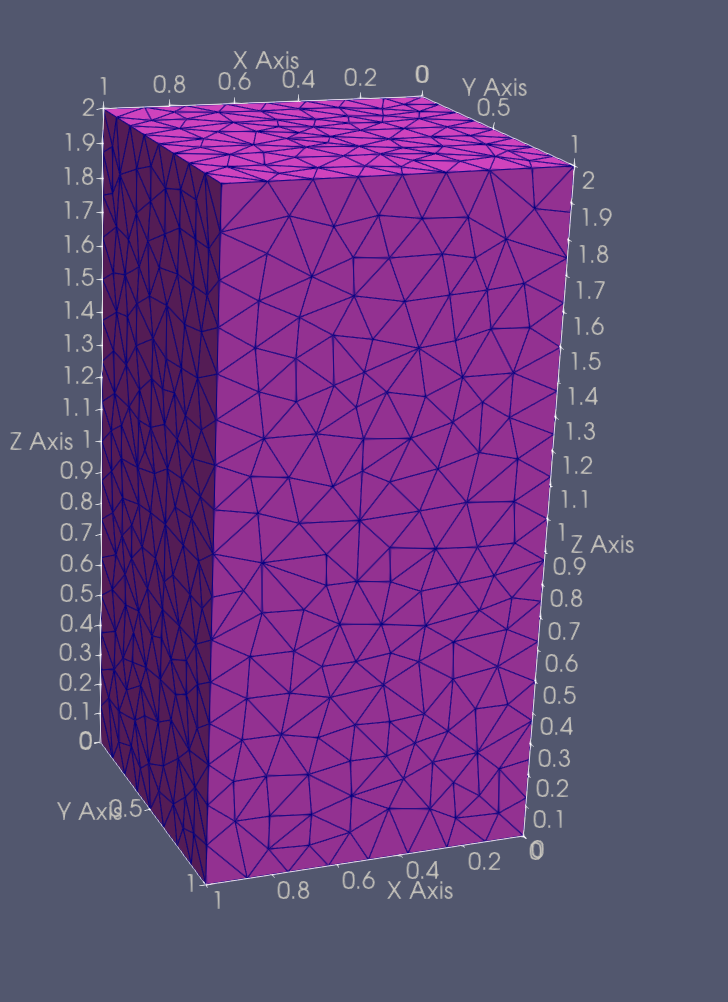
\includegraphics[width=0.9\linewidth]{images/prism.png}}
 	\caption{Сетка, с ограничением объема для тетраэдра 0.01. Визуализация в ParaView.}
 	\label{fig:prism}
\end{figure}

Таким образом работает построение сетки в MeshPy.

Рассмотрим теперь возможность перемещение объекта. Зададим сферу $S$ с помощью встроенной функции meshpy. Эта функция строит сферу с центром в (0,0,0). На вход можно изменить только два параметра сферы:
\begin{itemize}
    \item радиус
    \item количество разделений: в основу сферы берется окружность, которая вращается. Берется количесто разделений(кусков) $k$ и делится на $2\pi$. Получаем один интервал с полярной системе координат. Затем по окружности с шагом $\frac{2\pi}{k}$. Получается $k$ точек, принадлежащих окружности.
\end{itemize}

 \begin{figure}[H]
 	\center{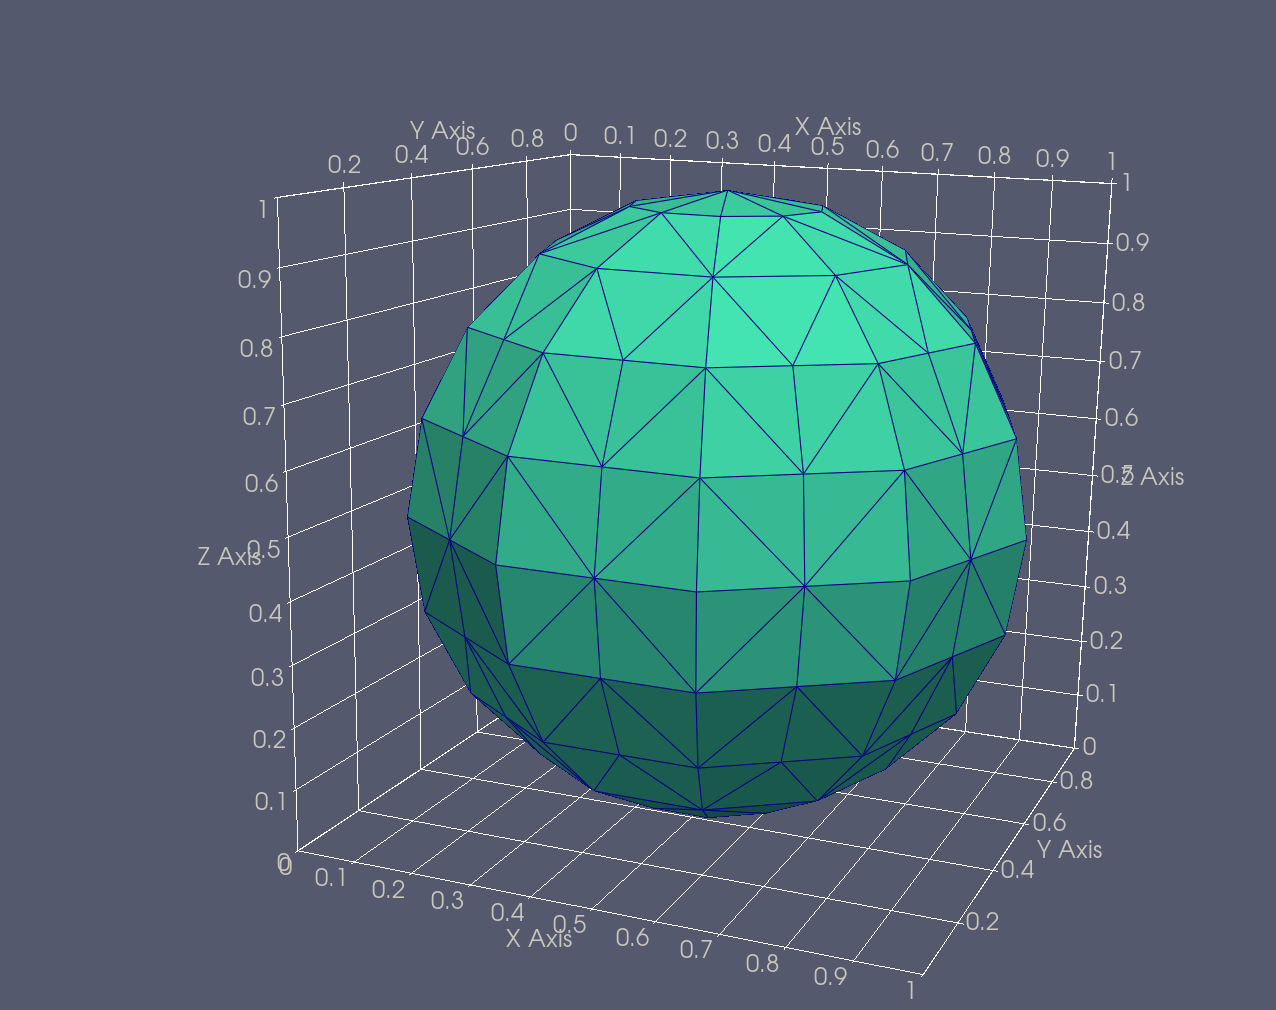
\includegraphics[width=0.9\linewidth]{images/sphere.png}}
 	\caption{Сетка, заполняющая сферу. Визуализация в ParaView. [Приложение Б]}
 	\label{fig:sphere}
 \end{figure}

У нас есть множество точек $\{point_{i}= (x_{i},y_{i},z_{i})\}\limits_{i = 1}^{n}$  и множество граней $\{facet_{j}\}\limits_{j = 1}^{m}$. Можно переместить сферу таким образом, чтоб ее центр находился в точке $a= (x_{a},y_{a},z_{a})$. Другими словами применить к множеству точек такую функцию:
 $$f(x,y,z) = (x,y,z) + (x_{a},y_{a},z_{a}).$$
Функция $f:~ \mathbb{R}^{3}\rightarrow \mathbb{R}^{3}$ линейна и не влияет никак на грани. Отношение и растояние между точками остается таким же. Поэтому можно переносить сферу в другие системы координат с другим центром. 

Аналогично можно превратить сферу в эллипсоид. Зададим функцию\\
$g:~\mathbb{R}^{3} \rightarrow \mathbb{R}^{3}$ таким образом:

\noindent
$$g(x,y,z) = (x,y,k~z),$$
где $k$ это какой-то коэффициент. Получим эллипсоид с радиусами $(r,r,k~r)$.
Это тоже не изменяет грани, потому что порядок точек остается таким же. 

Таким образом можно манипулировать сферой, чтоб получить другую фигуру и ее проанализировать. 

\section{Анализ фигуры}
Получув сетку фигуры, необходимо ее проанализировать, вычисляя следующие параметры:
\begin{itemize}
    \item Объем
    \item Площадь поверхности
    \item Центр масс
    \item Оценку сферичности
\end{itemize}

Для вычисления характеристик необходимо иметь координаты вершин тетраэдра. Как уже было сказано, после генерации сетки получаем объект с двумя полями: координатами и тетраэдрами. В списке тетраэдров хранятся индексы точек(индекс из списка точек). 

Пусть $ind_{k}, k = {1,4}$ --- индекс k-ой вершины тетраэдра, а $\{point_{i}= \}\limits_{i = 1}^{n}$ --- список точек. Тогда координата k-ой вершины можно найти таким образом:
$$ (x_{k},y_{k},z_{k}) = point_{ind_{k}}.$$

Зная координаты вершин, можно вычислить необходимые характеристики, подставляя их в функции [Приложение А].  

Но есть один метод вычисления площади поверхности, который можно применить именно в MeshPy. Как известно, для построение сетки необходимо задать грани фигуры. Грани это области принадлежащие $\mathbb{R}^{2}$. Так как сетки будут касаться этих границ, то площадь поверхности 
$$\mathscr{S}_{triangle} =\sum\limits_{j = 1}^{m} s(triangle_{j})$$
по треугольникам будет равнятся площади поверхности по граням
$$\mathscr{S}_{facet} =\sum\limits_{k = 1}^{b} s(facet_{k}).$$

Если посмотреть на визуализацию сетки и фигуры, то можно увидеть, что грани разделяются на треугольники, которые являются гранями тетраэдров сетки. Таким образом это утверждение имеет место. 

Площадь грани можно посчитать, разбив грань на треугольники и сложив их площади. В данном контексте рассматривается сфера, у которой грани являются треугольники и четырехугольники. Таким образом можно найти площадь поверхности, разбивая каждый четырехугольник на два треугольника. Важно учесть то, что трегульники должны всего лишь иметь общее ребро, поэтому нужно знать как MeshPy задает такие грани.

Такие грани задаются следующим образом: последовательно по часовой стрелке.

Пусть $pt = \{A,B,C,D\} $ - последовательные вершины четырехугольника, то есть ребра $\{AB,BC,CD,DA\}$ задают четырехугольник. Тогда площадь четырех угольника 
$$\mathscr{S}_{ABCD} = \mathscr{S}_{\triangle ABC} +  \mathscr{S}_{\triangle ACD}.$$
Треугольники $\triangle ABC$ и $\triangle ACD$ не пересекаются и имеют общее ребро. 
\section{Анализ последовательности эллипсоидов}
Зададим последовательность из десяти эллипсоидов с центром в (0,0,0) таким образом: 

$$ E_{k}: \frac{x^{2}}{a^{2}} + \frac{y ^{2}}{a^{2}} + \frac{z^{2}}{b^{2}} - 1 = 0, b = \frac{a}{k}, k = \{1,10\}. $$
Получается, что сфера сжимается с каждым шагом. 
\begin{figure}[H]
	\centering
	\label{fig:A}
	\subfigure[]{\label{fig:1}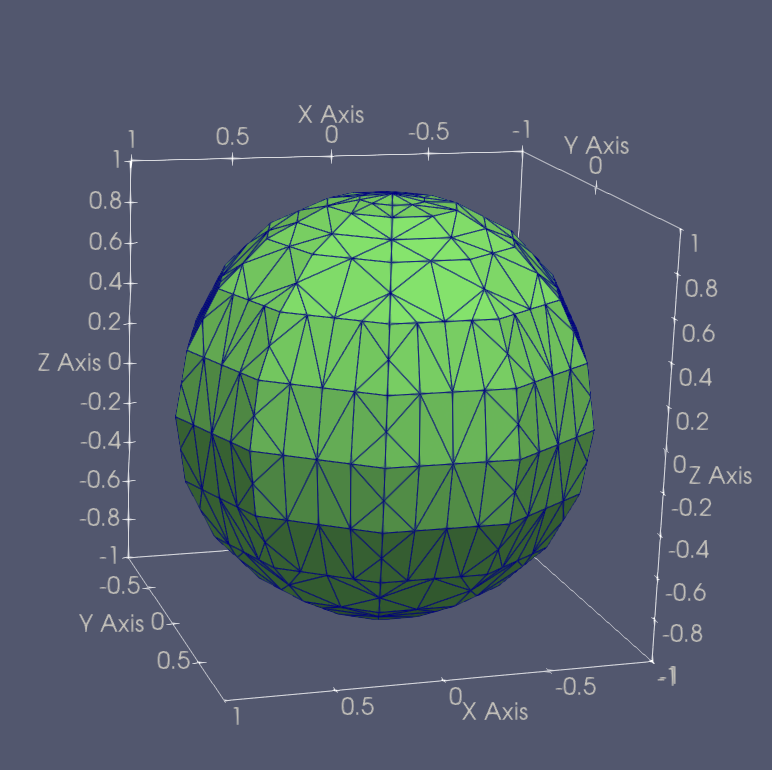
\includegraphics[width=0.4\linewidth]{images/ellipse1.png}} \\
	\subfigure[]{\label{fig:3}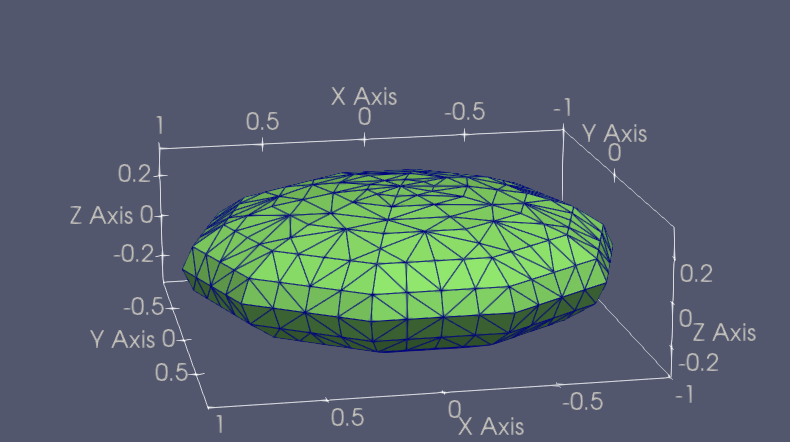
\includegraphics[width=0.4\linewidth]{images/ellipse3.png}} 
	\subfigure[]{\label{fig:6}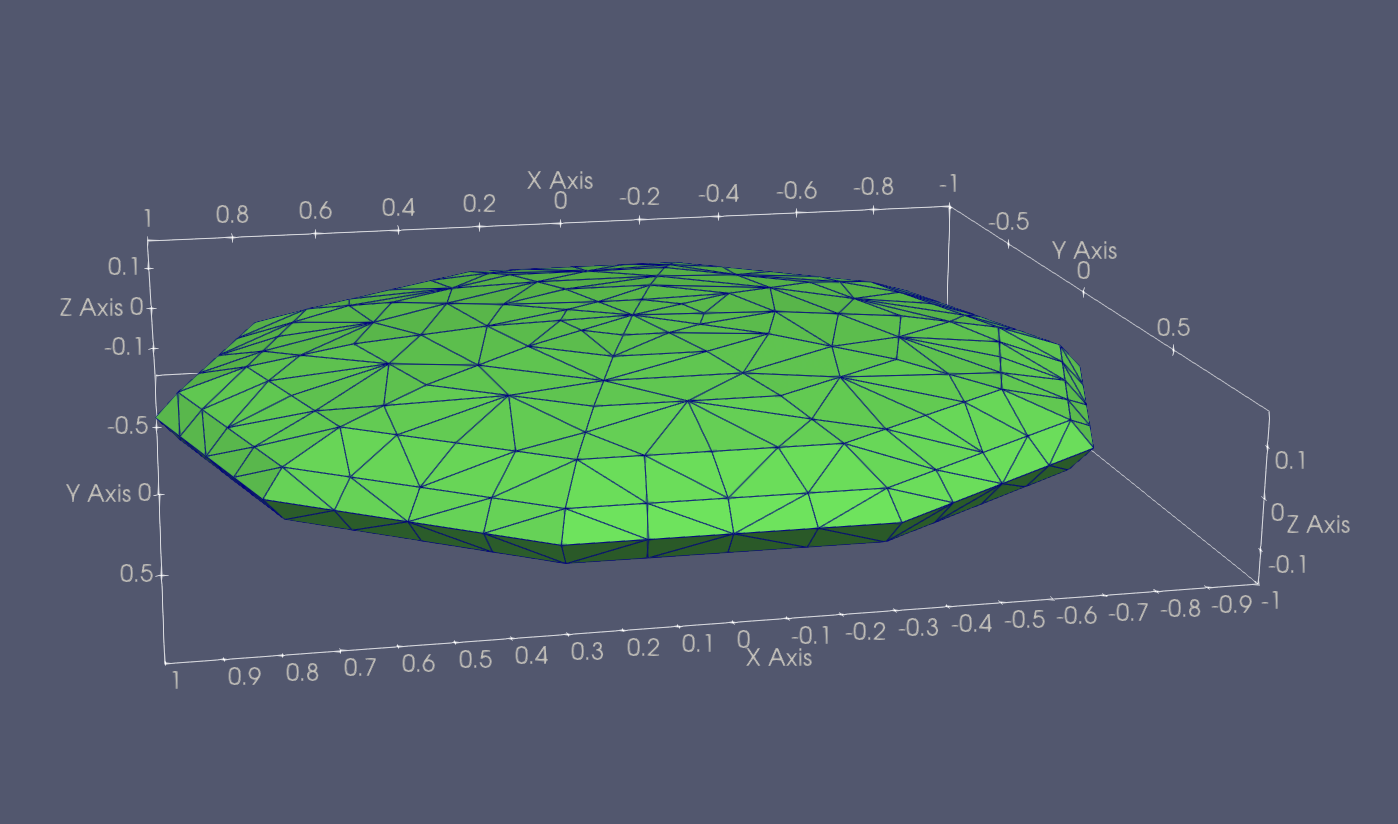
\includegraphics[width=0.4\linewidth]{images/ellipse6.png}}\\
	\caption{Эллипсоиды при k = 1(а),k = 3 (b),k = 6 (c).}
\end{figure}
Построим для каждого эллипсоида сетку и вычислим необходимые характеристики [Приложение В].
\begin{figure}[H]
	\centering
	\label{fig:B}
	\subfigure[]{\label{fig:ar}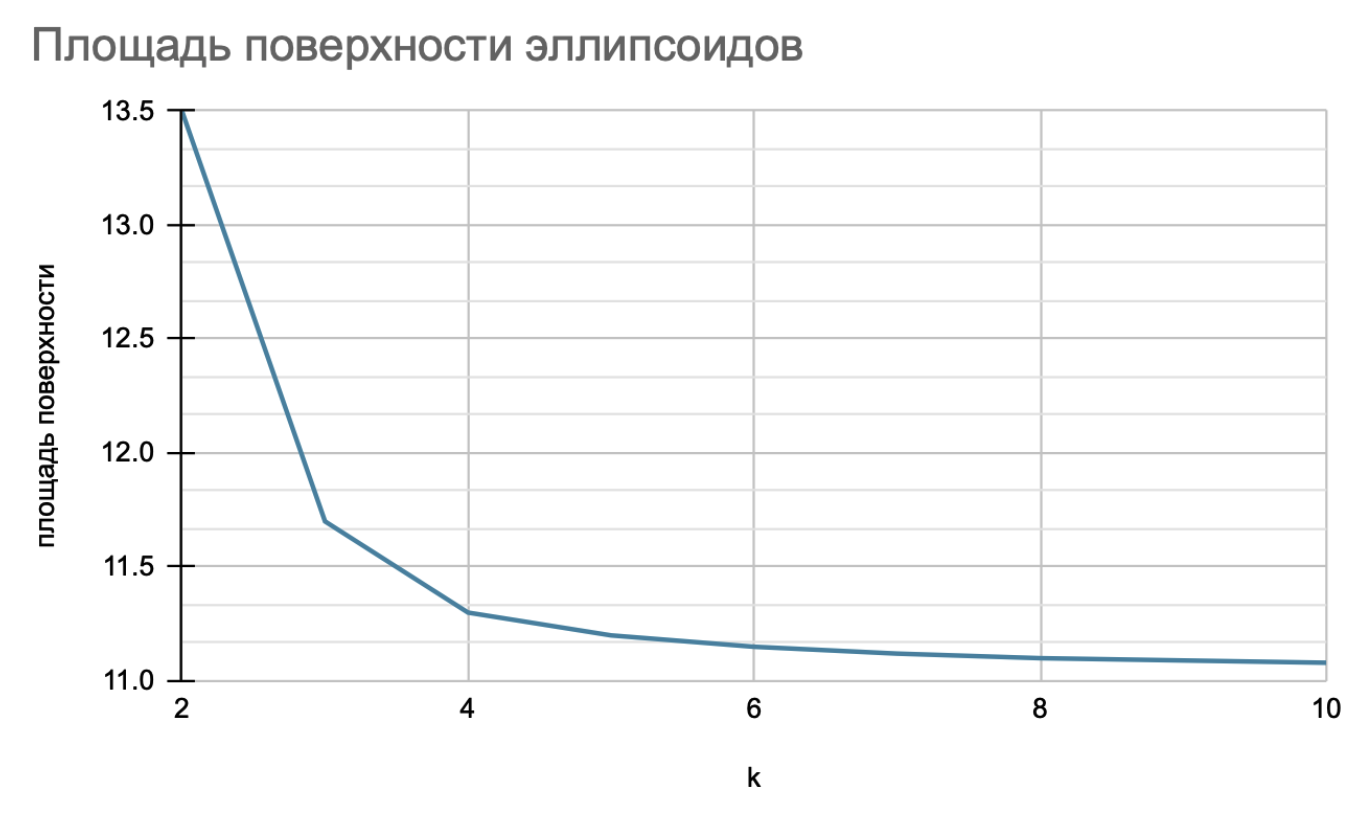
\includegraphics[width=0.6\linewidth]{images/area.png}}\\
	\subfigure[]{\label{fig:vol}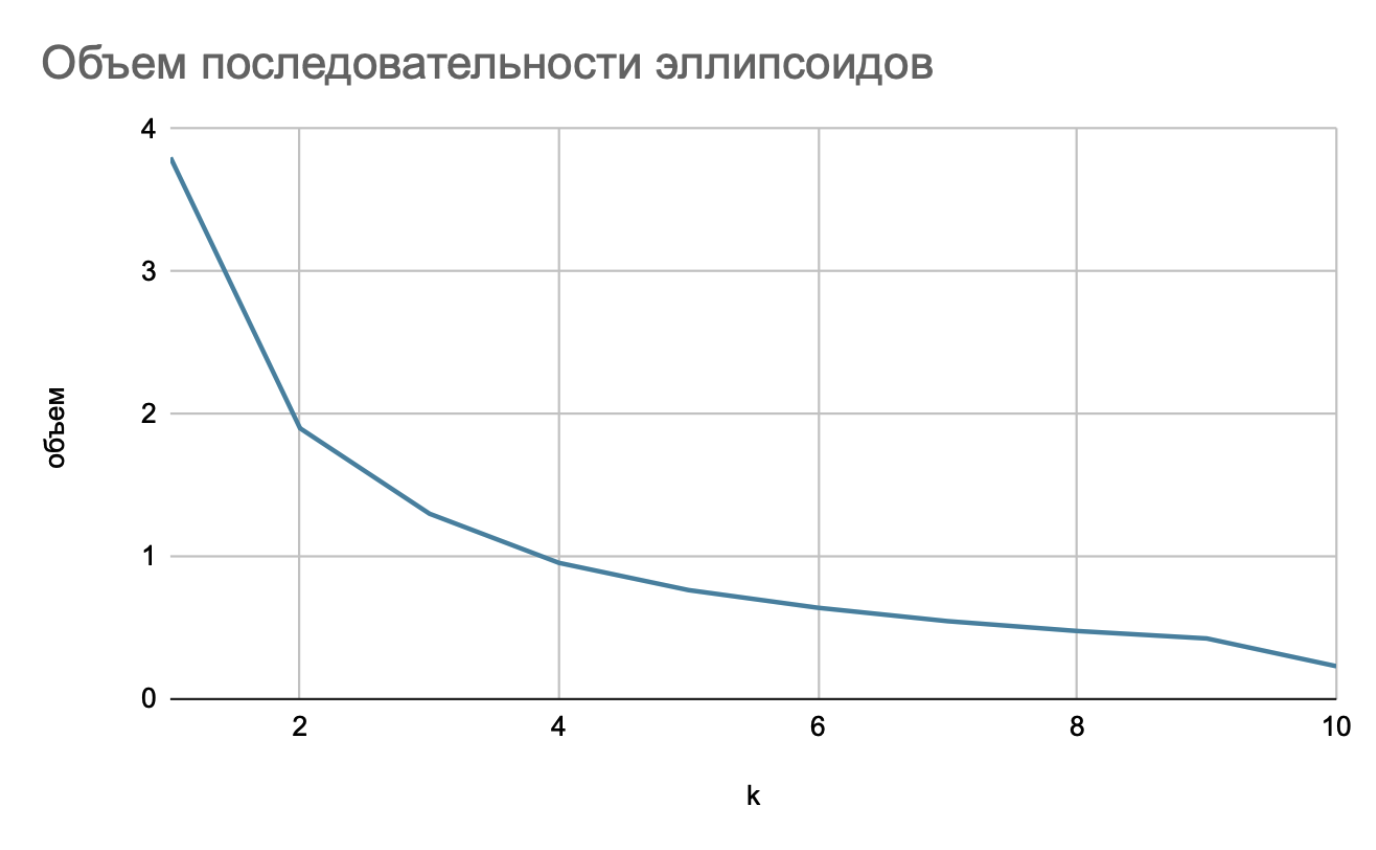
\includegraphics[width=0.6\linewidth]{images/volume.png}} \\
	\subfigure[]{\label{fig:sph}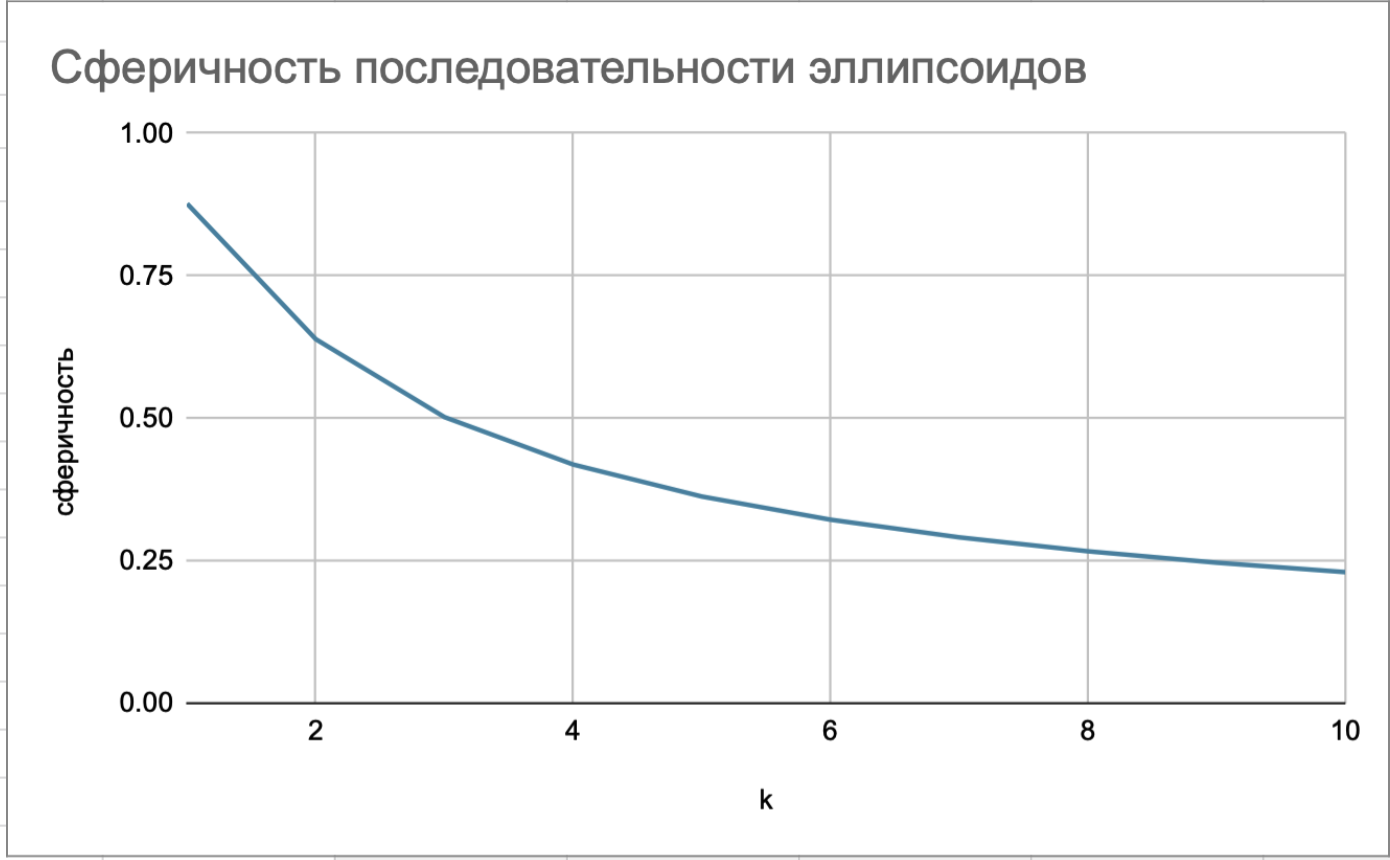
\includegraphics[width=0.6\linewidth]{images/sphericity.png}}
	\caption{Площадь поверхности(a), объем(b) и сферичность(c) последовательности эллипсоидов.}
\end{figure}

Как можно заметить, все параметры уменьшаются почти с той же динамикой. Центр масс для каждой фигуры в окрестности нуля. Так как данные были посчитаны питоном, возможно что там (0,0,0), но питон представляет это число как достаточно маленькое. Но, не исключено, что такая погрешность из-за неточности в объеме. Данная фигура вписана в эллипсоид и ее объем меньше объема самого эллипсоида.

Возьмем для примера сферу, то есть первый эллипсоид, где $ k = 1$ и радиус равен а(в данном случае 1). Вычислим объем и площадь поверхности. 

$$ \mathscr{V}_{sphere} = \frac{4}{3}\pi r^{3} = \frac{4}{3}\pi \approx  4.1889$$
$$ \mathscr{S} _{sphere} = 4 \pi r^{2} \approx 12.5664$$
Объем больше, чем у полученного, а площадь меньше (см.~ рис.\ref{fig:ar},\ref{fig:vol}). 

\chapter{АНАЛИЗ НЕСОГЛАСОВАННЫХ СЕТОК}
\section{Общая формулировка задачи}


Пусть известны два объекта: 
\begin{itemize}
    \item Сетка состоящая из тетраэдров $\Omega$.
    \item Другая сетка $\Gamma $, которая находится внутри первой сетки(она задана уравнением $f(x,y,z) = 0$). Ее внутренняя область обозначается как $\Omega_{\-}$
\end{itemize}
Необходимо изучить внутреннюю сетку и вычислить 4 характеристики по формулам с помощью сеток.  
В качестве примера рассмотрим начальное положение капли в двухфазном течении \cite[c.~34]{ns}. 
$$\Gamma_{0} =\{(x,y,z)\in \mathbb{R}^{3},  \|(x,y,z) - (\frac{1}{2},\frac{1}{2},\frac{1}{2}) \| = \frac{1}{4}\} $$
--- сфера,
$$ \Omega = [0,1]\times [0,1] \times [0,2] \in \mathbb{R}^{3}$$
--- прямоугольная призма.
Так как известно, как строить и анализировать сферу саму по себе, то можно построить две отдельные сетки. Для сферы посчитаны ее параметры.

\begin{figure}[H]
 	\center{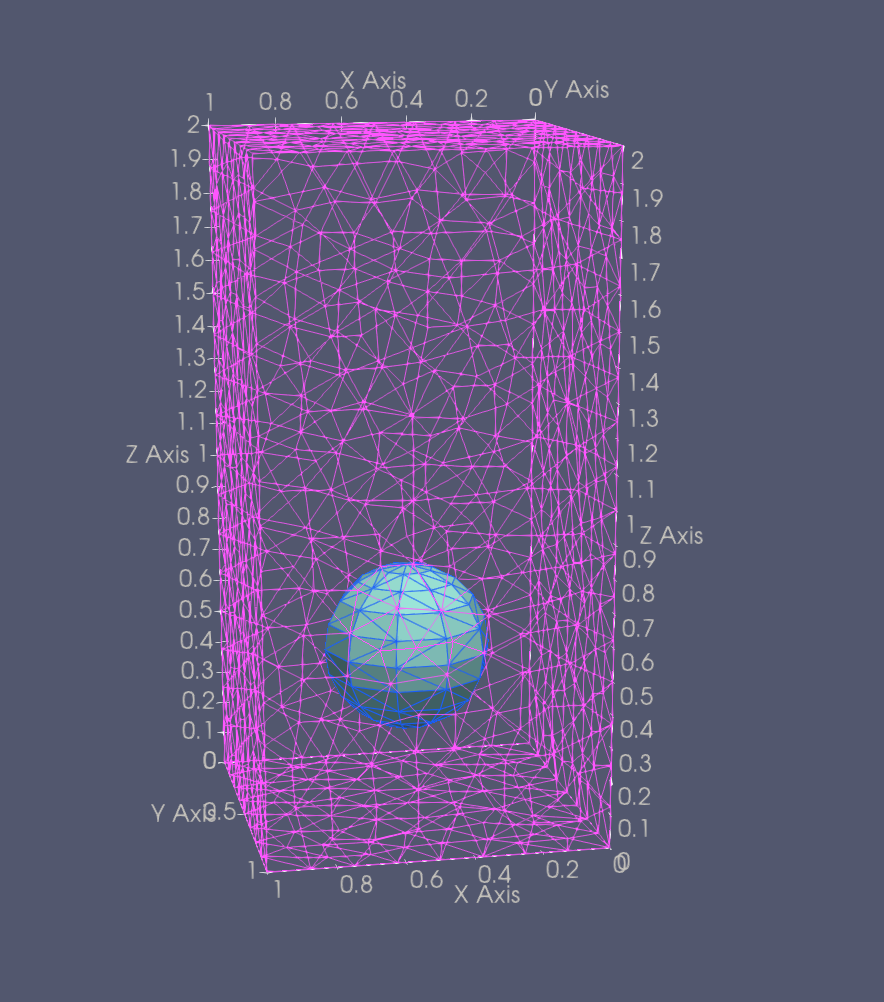
\includegraphics[width=0.9\linewidth]{images/problem.png}}
 	\caption{Геометрическое представление задачи. Построены две сетки. Визуализация в ParaView.}
 	\label{fig:problem}
\end{figure}

Но по условии задачи $\Gamma$ меняется со временем и фигура преобразится из сферы в другую. Необходима придумать решение для данных задач:
\begin{itemize}
    \item Как, зная уравнение поверхности $\Gamma$, найти область $\Omega_{-} \in \Omega$, которая является внутренней областью внутренней сетки? 
    \item Как посчитать характеристики для $\Gamma$?
\end{itemize}

\section{Метод выбора тетраэдров}

Так как известно, что фигура, границу которой задает $\Gamma$ находится в  $\Omega$, значит в фигуре содержатся тетраэдры, которые заполняют $\Omega$. Эти тетраэдры $t\in \Omega_{-}$. 

Рассмотрим пример со сферой в призме. Радиус нашей сферы равен $ r = \frac{1}{4}$, центр находится в точке $a = (\frac{1}{2},\frac{1}{2},\frac{1}{2}) $ . Тогда можно $\Gamma$ уравнением 
$$f(x,y,z) = (x-\frac{1}{2})^{2} + (y-\frac{1}{2})^{2} + (z-\frac{1}{2})^{2} - \frac{1}{16} = 0.$$

По определению, сфера это множество точек, которые равноудаленны от фиксированной точки. Получается, что те точки, которые лежат в сфере удалены от фиксированной точки $(x_{c},y_{c},z_{c})$ на растоянии $d < r$. Тогда 
$$f(x,y,z) = (x-x_{c})^{2} + (y-y_{c})^{2} + (z-z_{c})^{2} - r^{2} = d^{2} - r^{2} = (d - r)(d+r) < 0.$$

Следовательно, для того, чтоб тетраэдр полностью лежат во внутренней области $ \Omega_{-}$: 
$$\forall i \in \{1,4\} : f(x_{i},y_{i},z_{i}) < 0.$$
Если допустить, что тетраэдр касается границы $\Gamma$, то знак будет нестрогий.

Таким образом можно найти множестви тетраэдров $ T_{and} = \{t| t \in \Omega_{-}\}.$ 

К этому множеству можно применить формулу для вычисления характеристик. Но будут значительные погрешности, потому что сетки несогласованны. Это значит, что есть еще и тетраэдры, которые пересекают $\Gamma$, но не обязательно лежат в области $\Omega_{-}$. 

Таким образом можно найти еще одно множество тетраэдров по данному критерию: тетраэдр пересекается с областью $\Omega_{-}$, если хотя б одна его вершина удовлетворяет равенству $f(x,y,z) < 0$. 
$$\exists i \in \{1,4\} : f(x_{i},y_{i},z_{i}) < 0. $$
Назовем такое множество $ T_{or}$.

Индекс and означает то, что в условном блоке кода, где проверяется тетраэдр, все значения $f(x_{i},y_{i},z_{i}), i = {1,4}$ должны удовлетворять условию, чтоб тетраэдр принадлежал множеству(and используется как союз в блоке if) [Приложение Г].

Индекс or означает то, что в условном блоке кода, где проверяется тетраэдр, хотя б одно значение $f(x_{i},y_{i},z_{i}), i = {1,4}$ должно удовлетворять условию, чтоб тетраэдр принадлежал множеству (or используется как союз в блоке if) [Приложение Г].

В обоих множествах будут значительные погрешности:
\begin{itemize}
    \item у $T_{and}$ объем будет меньше.
    \item у $T_{and}$ объем будет больше.
\end{itemize}
Получается, что объем $\mathscr{V}(T_{or})$ является верхим пределом, а  $\mathscr{V}(T_{and})$ --- нижним.

При уменьшении объема(размера) тетраэдров в сетке $\Omega$ 
$$v \rightarrow 0,$$ количество тетраедров будет возрастать
$$n \rightarrow 0,$$
а объемы множеств $T_{or}$ и $T_{and}$ будут стремится к объему области $\Omega_{-}$. 
$$ \lim_{v\to 0 }\mathscr{V}(T_{and}) = \mathscr{V}(\Omega_{-})$$
$$ \lim_{v\to 0 }\mathscr{V}(T_{or}) = \mathscr{V}(\Omega_{-})$$

Единственная проблема увеличения количества тетраэдров --- увеличится время вычислений, потому что питон очень медленный в огромных итерациях. 


Метод выбора тетраэдров не самый лучший, потому что те тетраэдры, которые пересекаются с поверхностью $\Gamma$, либо вообще не учитываются, либо учитываются полностью. Это неправильно, потому что скорее всего там лежит часть тетраэдра. Таким методом еще очень сложно посчитать площадь поверхности. Тут не будут находится треугольники на поверхности, потому что тут тетраэдры пересекаются. Поэтому для данных высчислений было взято значение по формуле.
\section{Метод выпуклой оболочки}

Для более точный вычислений, необходимо придумать как учесть часть пересекающих тетраэдров. Один из методов это метод нахождения выпуклой оболочки по точкам пересечения сетки $\Omega$ с поверхностью $\Gamma$.

Метод выплуклой оболочки состоит из следующих шагов:
\begin{enumerate}
    \item Находим тетраэдры, которые пересекаются с данной поверностью $\Gamma$ 
    \item Для каждого тетрэадра, найденного в предыдущем шаге, находим точки пересечения с $\Gamma$
    \item Находим выпуклую оболочку для множества точек пересечения
    \item Используем выпуклую оболочку как двух мерную сетку и вычисляем необходимые характеристики
\end{enumerate}

Возьмем критерий пересечения из Никукилна: многогранних пересекается с плоскостью тогда и только тогда когда две его точки лежат по разные стороны \cite[c.~81]{nikulin}.
Пусть задана функция $f(x,y,z) = 0$, которая задает поверхность $\Gamma$. Тогда две точки лежат на противоположных стороннах поверхности: 
$$sign(f(x_{1},y_{1},z_{1})) \neq sign(f(x_{2},y_{2},z_{2})).$$

Чтоб проверить на пересечение тетраэдр, необходимо вывести список его ребер. Всего у тетраэдра 6 ребер, поэтому просто сделать это вручную, задав индексы точек в каждом ребре. Затем каждое ребро проверяем на пересечение. Если одно ребро пересекается с $\Gamma$, значит тетраэдр пересекается. Эти тетраэдры(или их индексы) необходимо занести в отдельный список, чтоб потом ими воспользоваться. 

Каждое ребро тетраэдра является отрезком какой-то прямой. Зададим параметрическое уравнение прямой $\mathscr{L}$ по двух точкам $(x_{1},y_{1},z_{1})$ и $(x_{2},y_{2},z_{2})$:
$$\mathscr{L}=\left\{ \begin{array}{c}
        x = (x_{2} - x_{1})t + x_{1} \\
        y = (y_{2} - y_{1})t + y_{1}\\
        z = (z_{2} - z_{1})t + z_{1}
    \end{array}{} \right . .$$

Подставляя вместо x,y,z эти выражения получаем уравнение с неизвестной переменной t: 
$$\Gamma(t) = 
f((x_{2} - x_{1})t + x_{1},
(y_{2} - y_{1})t + y_{1},
(z_{2} - z_{1})t + z_{1}) = 0~.$$

Для сферы это будет выглядеть следующим образом:
$$((x_{2} - x_{1})t + x_{1}-\frac{1}{2})^{2} + 
((y_{2} - y_{1})t + y_{1}-\frac{1}{2})^{2}
+ ((z_{2} - z_{1})t + z_{1}-\frac{1}{2})^{2} - \frac{1}{16}.$$
Получается квадратное уравнение с двумя решениями. Его можно решить используя библиотеку sympy. Задается сначала переменная, потом в функцию передеается уравнение. В данном случае будет два решения но для ребра необходима одна потому что тетраэдр значительно меньше сферы и не может одно ребро пересекать ее дважды. Поэтому нужно ввести дополнительное условие для нахождения точки, которая лежит на отрезке [Приложение Д]. 

Критерий принадлежности точки к отрезку:
Пусть т. $c$ принадлежит отрезку $ab$. Тогда:
$$ \vec{ca}\cdot\vec{cb} < 0.$$
где $a$ и $b$ это концы отрезка. Таким образом находим множество точек пересечения [Приложение Д]. 
Для сокращения время вычисления можно совместить проверку на пересечение и нахождение точек пересечение: Если ребро тетраэдра пересекается с поверхностью, находится точка пересечения. 

Далее необходимо построить выпуклую оболочку, которая будет двухмерной сеткой для $\Omega_{-}$. Есть класс в пакете scipy, который называется\\ scipy.spatial.ConvexHull. Он включает в себя QHull. С помощью этого класса можно построить выпуклую оболочку. Этот класс еще удобен тем, что у объекта есть два поля: 
\begin{itemize}
    \item объем
    \item площадь поверхности
\end{itemize}
Это означает, что уже посчитаны две характеристики для фигуры, которую покрывает двухмерная сетка. В формуля сферичности подставляем эти два значения и вычисляем. 

Для вычисления центра масс необходимо иметь множество тетраэдров. Во время проверки на пересечение тетраэдры сетки делятся на две группы:
\begin{itemize}
    \item пересекаются с $\Gamma$
    \item не пересекаются
\end{itemize}
В качестве множества тетраэдров нужно взять тетраэдры, которые пересекаются. Но стоит обратить внимание, что нужно для этого множества сумму объемов посчитать. На каком-то этапе разработки была совершена ошибка, когда центр был поделен на объем фигуры в выпуклой оболочки. 
Центр масс оказался за пределами самой сетки. Чтоб исправить эту ошибку, необходимо посчитать объемов выбранных тетраэдров [Приложение Е]. 

Несмотря на время выполнение этот метод самый близкий к расчетом по известным гоеметрическим формулам. В таблице видно, что результат самый близким к значениям, посчитанным по известным геометрическими формулам для сферы \ref{table:1}.

\begin{table}[h]
\caption{Результаты разных методов вычиселния}
\label{table:1}
\centering 
\begin{tabular}{ |p{2cm}|p{2cm}|p{2cm}|p{2cm}| p{2cm}|p{2cm}| }
\hline
{}& Вычисле- ние по формулам
& Вычисле- ние отдельной сети & Выбор внутренних & Выбор внутренних и пересекающих & метод выпуклой оболочки \\
\hline
Объем & 0.065 & 0.06 & 0.015 & 0.134 & 0.06\\
\hline
Сферич- ность & 1 & 0.88 & 0.38 & 1.61 & 0.986\\
\hline
Центр масс & (0.5,0.5, 0.5) & (0.5,0.5 ,0.5)& (0.506, 0.508, 0.47)  &  (0.51, 0.506, 0.47) &  (0.509, 0.506, 0.47) \\
\hline
Время вычислений(сек) & 0 & 0.18 & 0.51 & 0.57 & 192 \\
\hline
\end{tabular}
\end{table}


